\documentclass[12pt, twoside]{article}
\usepackage[letterpaper, margin=1in, headsep=0.2in]{geometry}
\setlength{\headheight}{0.6in}
%\usepackage[english]{babel}
\usepackage[utf8]{inputenc}
\usepackage{microtype}
\usepackage{amsmath}
\usepackage{amssymb}
%\usepackage{amsfonts}
\usepackage{siunitx} %units in math. eg 20\milli\meter
\usepackage{yhmath} % for arcs, overparenth command
\usepackage{tikz} %graphics
\usetikzlibrary{quotes, angles}
\usepackage{graphicx} %consider setting \graphicspath{{images/}}
\usepackage{parskip} %no paragraph indent
\usepackage{enumitem}
\usepackage{multicol}
\usepackage{venndiagram}

\usepackage{fancyhdr}
\pagestyle{fancy}
\fancyhf{}
\renewcommand{\headrulewidth}{0pt} % disable the underline of the header
\raggedbottom
\hfuzz=2mm %suppresses overfull box warnings

\usepackage{hyperref}

\fancyhead[LE]{\thepage}
\fancyhead[RO]{\thepage \\ Name: \hspace{4cm} \,\\}
\fancyhead[LO]{BECA / Dr. Huson / Geometry\\*  Unit 12: Trigonometry \\* 24 March 2023}

\begin{document}

\subsubsection*{12.10 Test: Trigonometry \hfill HSG.SRT.C.8}
\begin{enumerate}
\item As shown, right $\triangle ABC$ has $AC=8, BC=15, AB=17$, $m\angle C=90^\circ$. \\[0.25cm] 
Express each trigonometric ratio as a fraction.
  \begin{multicols}{2}
    \begin{enumerate}[itemsep=0.2cm]
      \item $\sin A =$
      \item $\cos A =$
      \item $\tan A =$
      \item Find $m\angle A$.
    \end{enumerate}
    \begin{center}
      \begin{tikzpicture}[scale=0.6]
        \draw [thick](0,0) node[below]{$A$}--
        (4,0) node[below]{$C$}--
        (4,8) node[above right]{$B$}--cycle;
        \node at (2,0)[below]{$8$};
        \node at (4,4)[right]{$15$};
        \node at (2,4)[left]{$17$};
        \draw (4,0)++(-0.6,0)--++(0,0.6)--+(0.6,0);
        \draw (0.75,0) arc [start angle=0, end angle=63, radius=0.75];
      \end{tikzpicture}
    \end{center}
  \end{multicols} \vspace{1cm}

\item Right triangle $\triangle ABC$ is shown with measures as marked.\vspace{0.25cm}
\begin{multicols}{2}
  \begin{enumerate}[itemsep=0.5cm]
    \item Write down $\sin A$.
    \item Find the length of side $AC$.\vspace{1.5cm}
    \item Find the angle measure of $\angle A$.
    \vspace{1cm}
  \end{enumerate}
\begin{flushright}
        \begin{tikzpicture}[scale=1]
        \draw [thick]
        (0,0)node[left]{$A$}--
        (4,0)node[below right]{$C$}--
        (4,3)node[right]{$B$}--cycle;
        \draw (4,0)++(-0.5,0)--++(0,0.5)--+(0.5,0);
        \node at (4,1.5)[right]{$3$};
        \node at (1.9,1.8){$5$};
        %\node at (4,2.7)[right]{$8$};
        %\node at (1.8,2.6)[above]{$10$};
      \end{tikzpicture}
\end{flushright}
\end{multicols} \vspace{1.5cm}

\item Isosceles right $\triangle ABC$ is shown with legs $AC=BC=1$ as marked.\vspace{0.25cm}
  \begin{multicols}{2}
    \begin{enumerate}[itemsep=0.2cm]
      \item Write down $\theta$.
      \item Find the length of hypotenuse $AB$.\vspace{2cm}
    \end{enumerate}
    \begin{flushright}
      \begin{tikzpicture}[scale=0.7]
        \draw [thick](0,0)node[below]{$A$}--
        (5,0)node[below]{$C$}--
        (5,5)node[above right]{$B$}--cycle;
        \draw (5,0)++(-0.6,0)--++(0,0.6)--+(0.6,0);
        \node at (2.5,0)[below]{$1$};
        \node at (5,2.5)[right]{$1$};
        \draw [thick, -] (1,0) arc [start angle=0, end angle=45, radius=1];
        \node at (1.2,0.1)[above]{$\theta$};
      \end{tikzpicture}
    \end{flushright}
  \end{multicols} \vspace{1cm}

\newpage
\item Right $\triangle ABC$ has base $AC=1$, height $BC=\sqrt{3}$, and hypotenuse $AB=2$ as marked. (A reflection $\triangle ABC$ of is also shown.)\vspace{0.25cm}
\begin{enumerate}[itemsep=0.6cm]
  \begin{multicols}{2}
    \item Write down the angle measure of $\angle A$.
    \item Write down the angle measure of $\angle ABC$.
\item Write down $\cos A$.
\begin{flushright}
        \begin{tikzpicture}[scale=0.8]
        \draw [thick]
        (0,0)node[below]{$A$}--
        (3,0)node[below]{$C$}--
        (60:6)node[above]{$B$}--cycle;
        \draw (3,0)++(-0.5,0)--++(0,0.5)--+(0.5,0);
        \draw [dashed] (3,0)--(6,0)--(60:6);
        \node at (1.5,0)[below]{$1$};
        \node at (62:3)[left]{$2$};
        \node at (3,2)[right]{$\sqrt{3}$};
      \end{tikzpicture}
\end{flushright}
\end{multicols}
\end{enumerate}
\vspace{1cm}

\item At an angle of elevation of $17^\circ$, the top of a structure $B$ is visible from point $A$ on the ground 100 meters away, as shown below.

Find the height $h$ of the structure to the \emph{nearest meter}. \hfill (not to scale)
  \begin{flushright}
    \begin{tikzpicture}[scale=0.3]
      %\draw [-, thick] (0,0)--(35:23);
      \draw [-, thick] (-4,0)--
      (0,0)--
        (17,0)--
        (22,0)--
        (22,10)--(17,10)--(17,0);
      \draw [fill] (0,0) circle [radius=0.1] node[above left]{$A$};
      \draw [fill] (17,10) circle [radius=0.1] node[above right]{$B$};
      \draw [dashed] (0,0)--(17,10);
      \node at (3.8, 0)[above]{$17^\circ$};
      \node at (11, 0)[below]{100 m};
      \node at (17, 5)[right]{$h$};
    \end{tikzpicture}
    \end{flushright}

\item A 15-foot ladder leans against a building and reaches a window 12 feet above ground. What is the measure of the angle, to the \emph{nearest degree}, that the ladder forms with the ground?

\newpage
\item Are the lines parallel, perpendicular, or neither? Justify your answer. \\(you must use the values of the slopes in your justification)
  \begin{multicols}{2}
    $y = 2x+5$ \\
    $y = -\frac{1}{2}x-9$
  \end{multicols} \vspace{2cm}

\item Given $P(4,6)$ and $Q(1,12)$, find the length of $\overline{PQ}$, expressed as a simplified radical.\\[0.25cm]
Use: $l=\sqrt{(x_2-x_1)^2+(y_2-y_1)^2}$
    \vspace{6cm}

\item A translation $T_{x,y}$ maps $A(-3,5) \rightarrow A'(-7,8)$. 
\begin{enumerate}
  \item Write down the translation. \vspace{1cm}
  \item Apply the same translation to $B(5, 4)$.
\end{enumerate} \vspace{1.5cm}

\item In a right triangle, the acute angles have the relationship $\sin(2x + 7) =\cos (33)$. \\[0.25cm]
What is the value of $x$?

\newpage
\item In the diagram below, $\overline{PQ}$ has endpoints with coordinates $P(1,5)$ and $Q(7,1)$. Find the equation of the perpendicular bisector of $\overline{PQ}$ and plot it on the grid.
  \begin{flushright}
    \begin{tikzpicture}[scale=.48]
      \draw [help lines] (-5,-5) grid (9,7);
      \draw [thick, <->] (-5.4,0) -- (9.4,0) node [below right] {$x$};
      \draw [thick, <->] (0,-5.4)--(0,7.4) node [left] {$y$};
      \draw [thick] (1,5)--(7,1);
      \draw [fill] (1,5) circle [radius=0.1] node[above left] {$P$};
      \draw [fill] (7,1) circle [radius=0.1] node[above right] {$Q$};
    \end{tikzpicture}
  \end{flushright} \vspace{3cm}

\item In the diagram below, $\triangle ABC$ is inscribed in semi-circle $O$. Show that $\overline{AB} \perp \overline{BC}$.
    \begin{flushright}
      \begin{tikzpicture}[scale=0.6]
        \draw [help lines] (0,0) grid (10,7);
        \draw [thick, <->] (-0.4,0) -- (10.4,0) node [below right] {$x$};
        \draw [thick, ->] (0,0)--(0,7.4) node [left] {$y$};
        \draw [thick]
          (0,0)node[below]{$A$}--
          (8,4) node[above right]{$B$}--
          (10,0) node[below]{$C$}--cycle;
        \draw [fill] (5,0) circle [radius=0.1] node[below] {$O$};
        \clip (0,0) rectangle (10,6);
        \draw (5,0) circle [radius=5];
      \end{tikzpicture}
    \end{flushright} \vspace{1cm}

\newpage
\item As shown in the diagram below, quadrilateral $ABCD$ has vertices with coordinates $A(1,2)$, $B(5,5)$, $C(5,0)$, and $D(1,-3)$.\\[0.25cm]
Show that $ABCD$ is a rhombus.
\begin{enumerate}
  \item Find the lengths of the sides of $ABCD$.
    \begin{flushright}
      \begin{tikzpicture}[scale=0.6]
        \draw [help lines] (-2,-5) grid (7,7);
        \draw [thick, <->] (-2.4,0) -- (7.4,0) node [below right] {$x$};
        \draw [thick, <->] (0,-5.7)--(0,7.4) node [left] {$y$};
        \draw [thick]
          (1,2)node[above left]{$A$}--
          (5,5) node[right]{$B$}--
          (5,0) node[above right]{$C$}--
          (1,-3) node[below right]{$D$}--cycle;
      \end{tikzpicture}
    \end{flushright} \vspace{3cm}
    \item Write a concluding statement using the definition that a quadrilateral is a rhombus if and only if its four sides are congruent.
  \end{enumerate}


\end{enumerate}
\end{document}
  